\documentclass[]{article}
\usepackage{indentfirst}
\usepackage{graphicx}
\usepackage{float}

%opening
\title{Operating Systems Problem session 2}
\author{Dibran Dokter 1047390 \& Marnix Lukasse 1047400}

\begin{document}

\maketitle

\subsection*{5.2}
\begin{bfseries} Question: \end{bfseries}\\
Discuss how the following pairs of scheduling criteria conflict in certain
settings.\\
a. CPU utilization and response time\\
b. Average turnaround time and maximum waiting time\\
c. I/O device utilization and CPU utilization\\
\begin{bfseries} Answer: \end{bfseries}\\
a. When the CPU is utilised 100\% then the system is unable to schedule any new processes and thus the new processes will have to wait a long time and the response time will suffer.\\
b. Some algorithms can give a relatively low turnaround time but that often means that some (long) processes have a very long waiting time.\\
c. When there is a CPU-heavy process using alot of the CPU then the CPU utilization can be good, it could cause for a convoy effect however. In that case the other processes are stuck in the ready queue waiting to get their CPU-burst. Only then they will be able to do a I/O-burst again. So this can cause bad I/O utilization.\\

\subsection*{5.5}
\begin{bfseries} Question: \end{bfseries}\\
Consider the exponential average formula used to predict the length of
the next CPU burst. What are the implications of assigning the following
values to the parameters used by the algorithm?\\
a. $\alpha$ = 0 and $\tau_0$ = 100 milliseconds\\
b. $\alpha$ = 0.99 and $\tau_0$ = 10 milliseconds\\
\begin{bfseries} Answer: \end{bfseries}\\
a. In this case $\tau_0$ is used. Thus we dont take the history into account and only rely on the original prediction.\\
b. In this case $\tau_0$ has almost no impact but the average of the other values count for 0.99. So in this case the estimated time is strongly impacted by the very recent history (past cycle).\\
\subsection*{5.7}\
\begin{bfseries} Question: \end{bfseries}\\
Consider the following set of processes, with the length of the CPU burst
given in milliseconds:\\
\begin{tabular}{|l|l|l|}
Process & Burst Time & Priority\\
\hline
P1 & 2 & 2 \\
\hline
P2 & 1 & 1 \\
\hline
P3 & 8 & 4 \\
\hline
P4 & 4 & 2 \\
\hline
P5 & 5 & 3 \\
\end {tabular}

The processes are assumed to have arrived in the order P 1 , P 2 , P 3 , P 4 , P 5 ,
all at time 0.\\

a. Draw four Gantt charts that illustrate the execution of these pro-
cesses using the following scheduling algorithms: FCFS , SJF , non-
preemptive priority (a larger priority number implies a higher
priority), and RR (quantum = 2).\\
b. What is the turnaround time of each process for each of the
scheduling algorithms in part a?\\
c. What is the waiting time of each process for each of these schedul-
ing algorithms?\\
d. Which of the algorithms results in the minimum average waiting
time (over all processes)?\\

\begin{bfseries} Answer: \end{bfseries}\\
a.\\

\begin{figure}[H]
  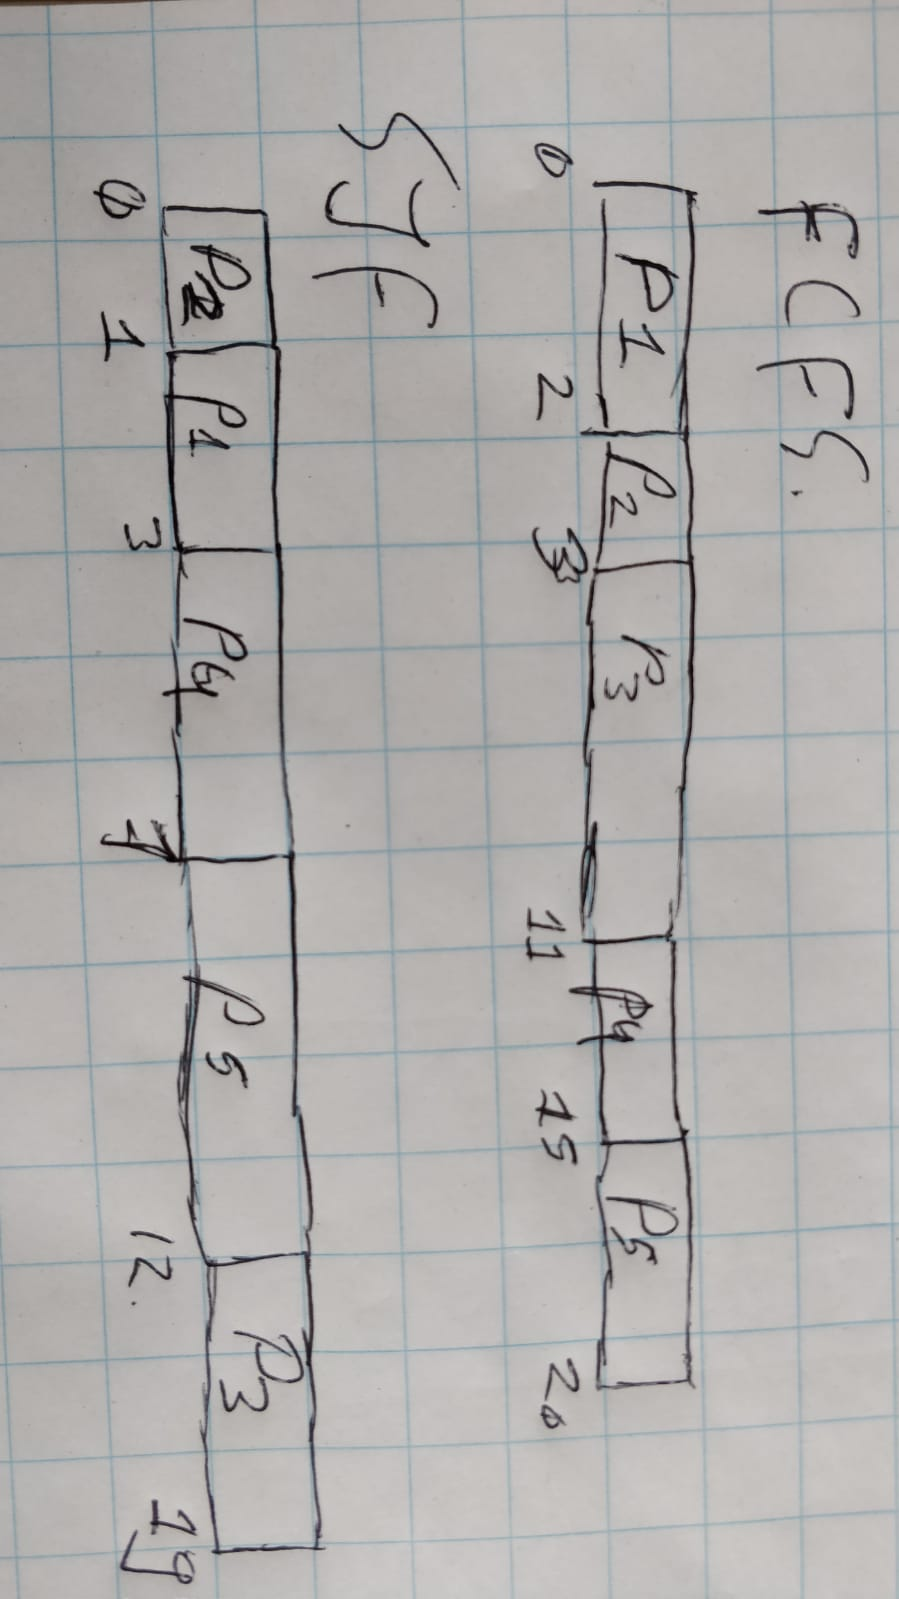
\includegraphics[width=\linewidth]{/home/owner/git/operatingsystems/week2/images/gannt1.jpeg}
\end{figure}

\begin{figure}[H]
  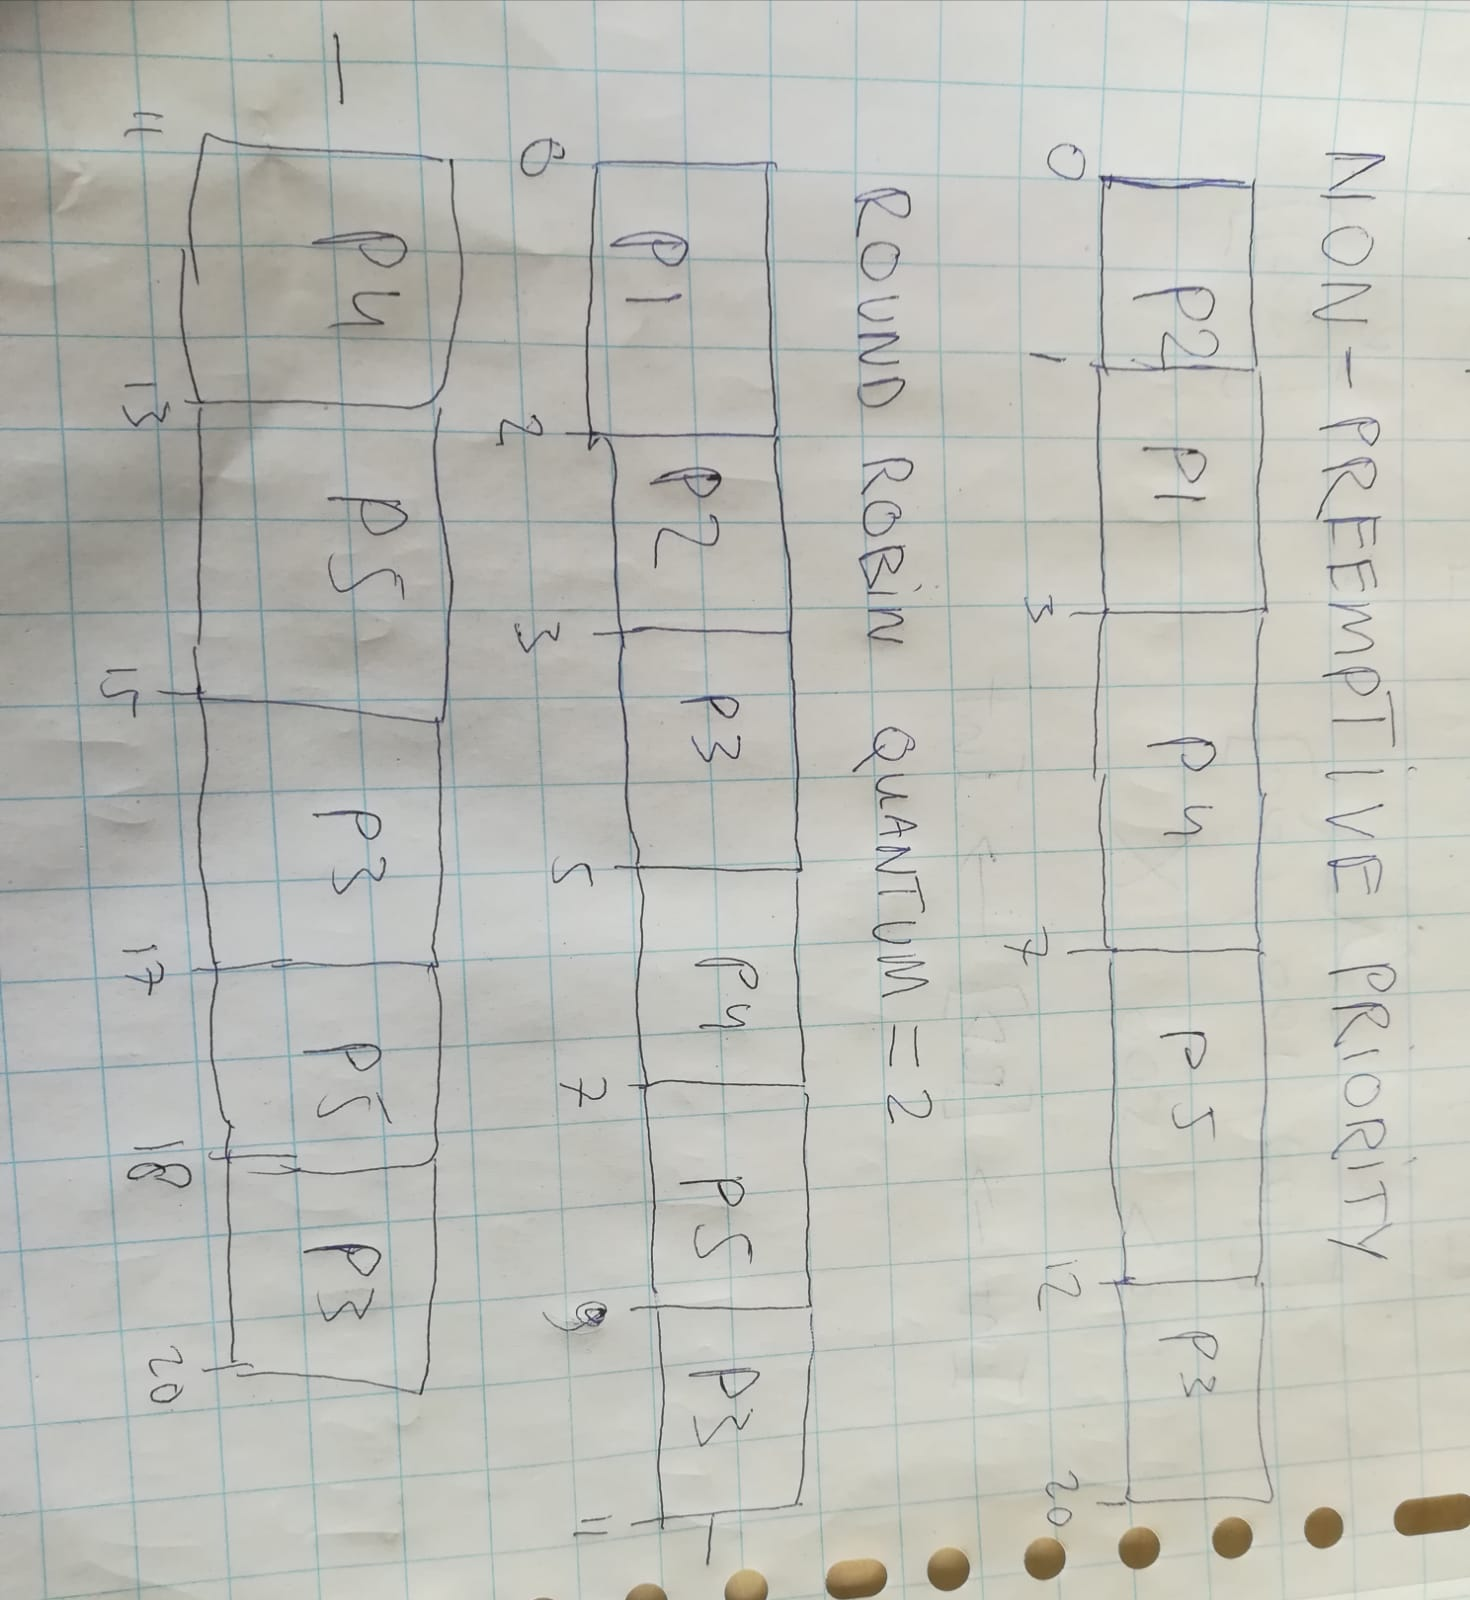
\includegraphics[width=\linewidth]{/home/owner/git/operatingsystems/week2/images/gannt2.jpeg}
\end{figure}
 
b \& c.
  
\begin{figure}[H]
  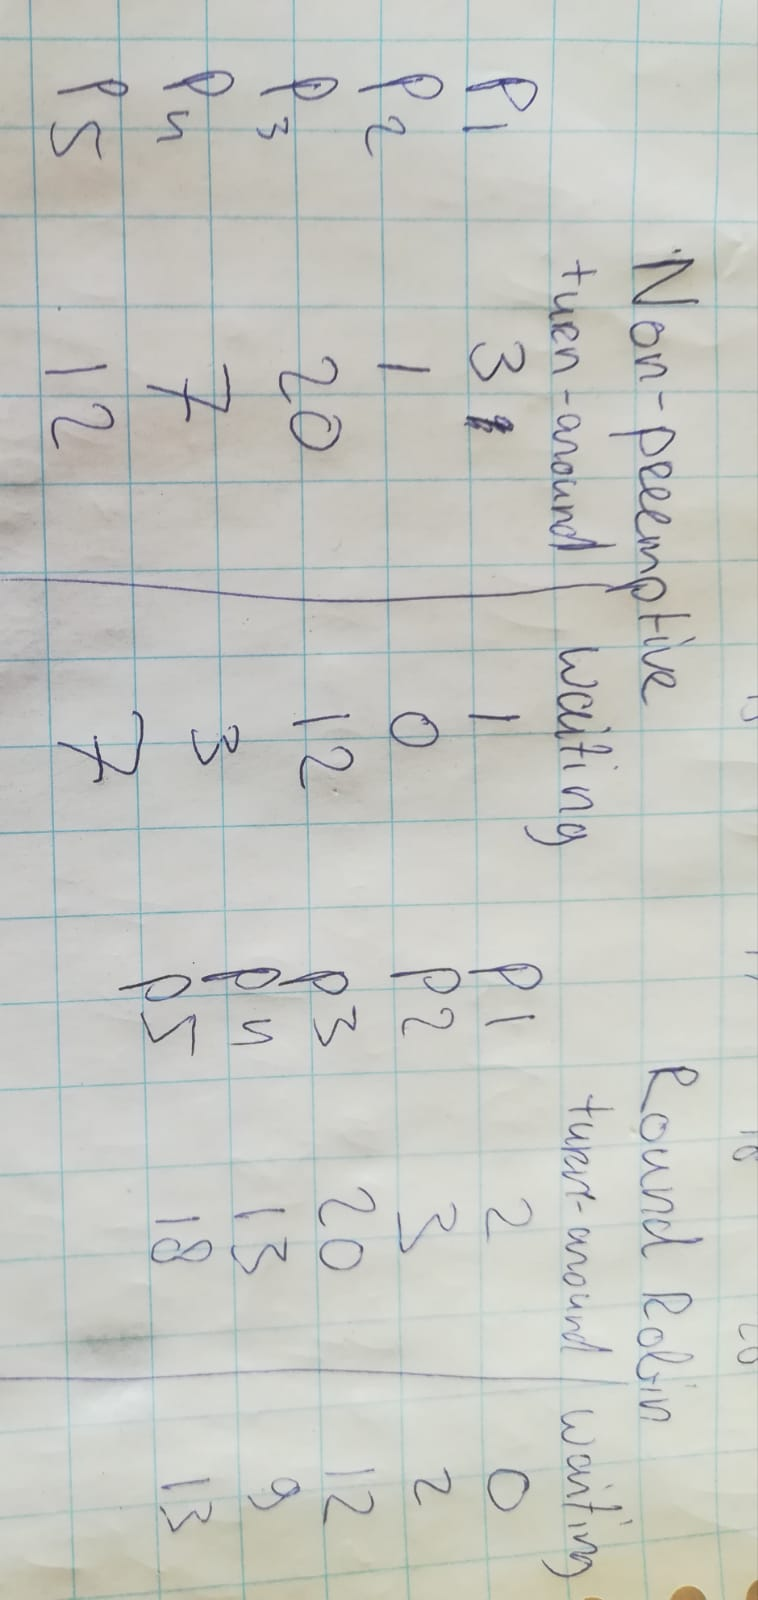
\includegraphics[width=\linewidth]{/home/owner/git/operatingsystems/week2/images/table1.jpeg}
\end{figure}

\begin{figure}[H]
  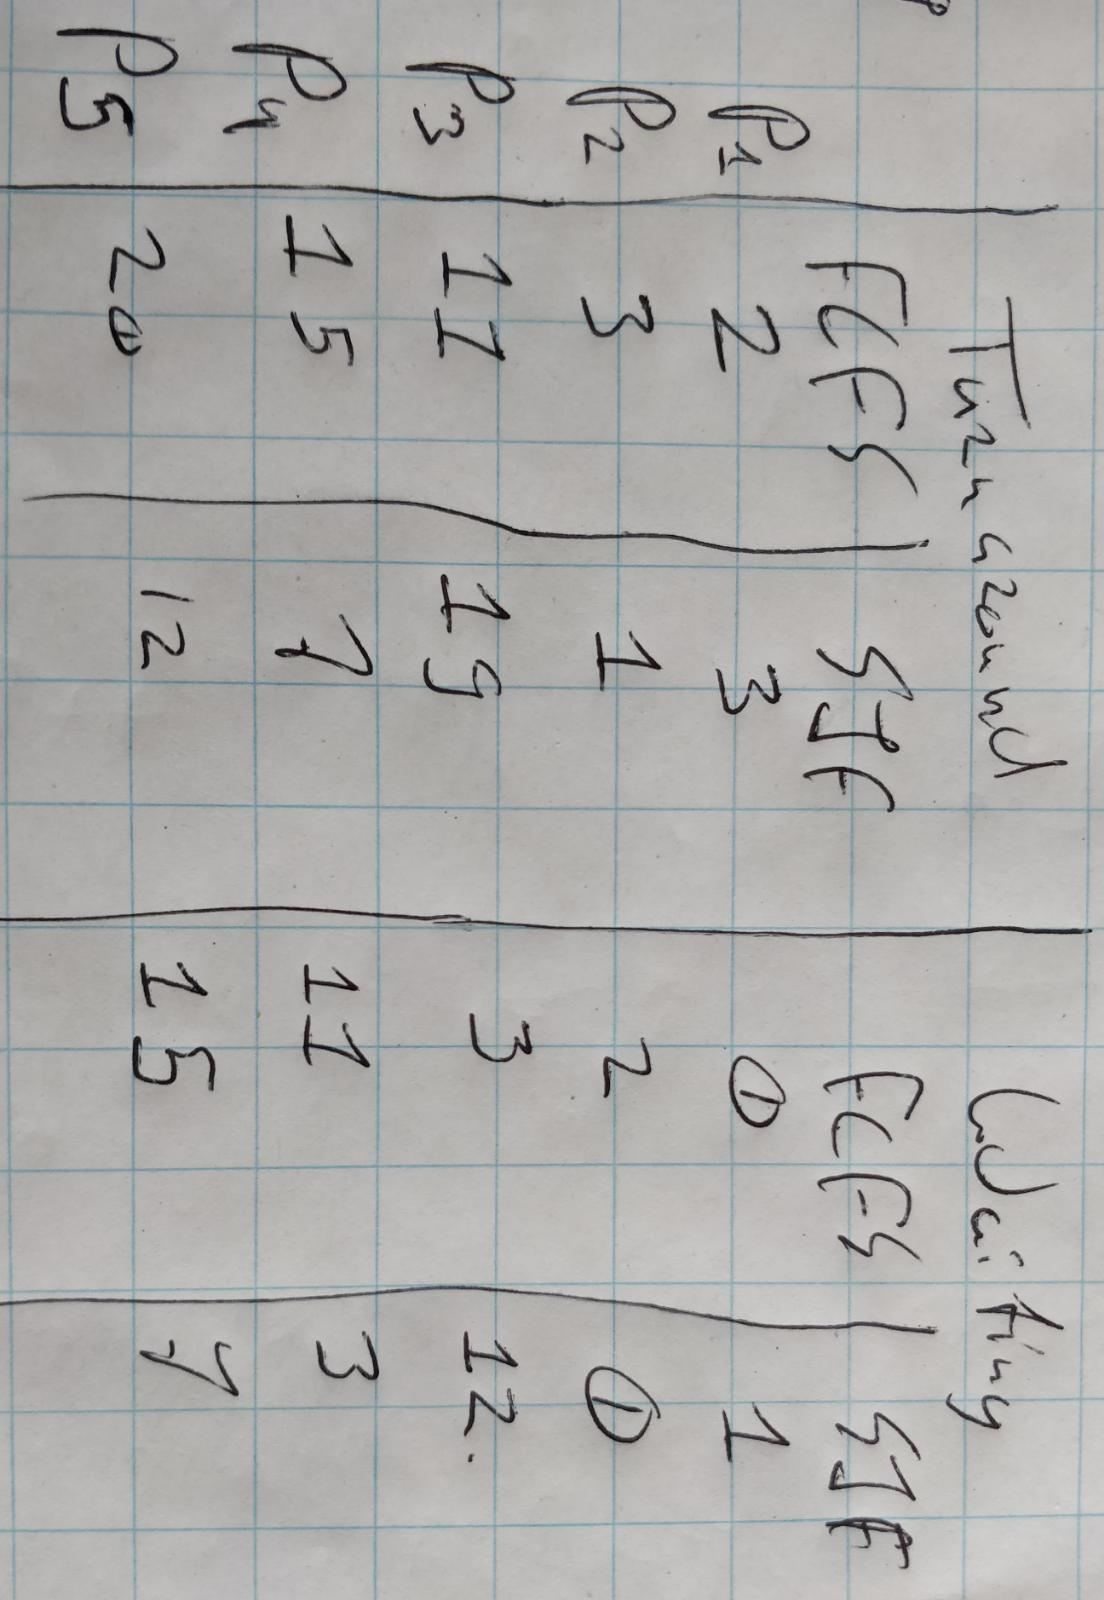
\includegraphics[width=\linewidth]{/home/owner/git/operatingsystems/week2/images/table2.jpeg}
\end{figure}

d. Non-preemtive and priority and SJF have the same waiting time of 4.6. This is the lowest average waiting time.

\subsection*{5.8}

a \& b \& c.
\begin{figure}[H]
  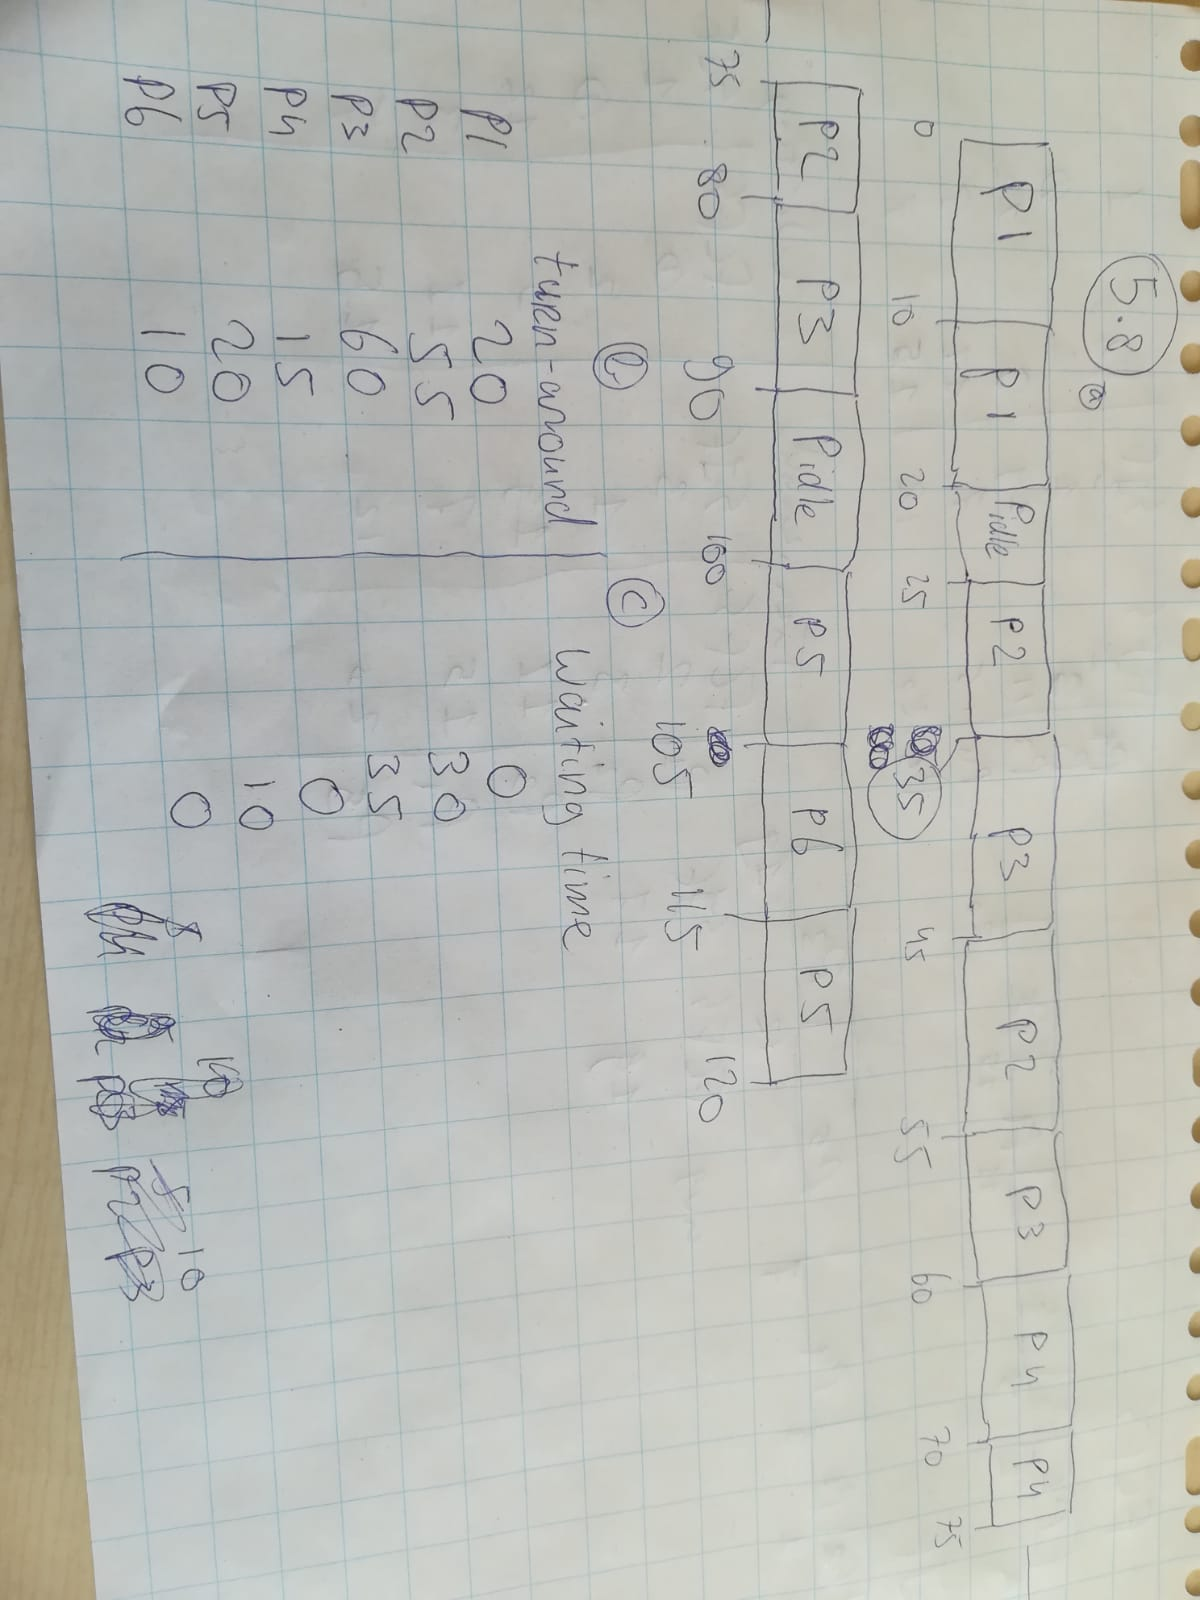
\includegraphics[width=\linewidth]{/home/owner/git/operatingsystems/week2/images/gannt3.jpeg}
\end{figure}

d. 87.5\%,\\ (105 / 120 * 100)

\subsection*{5.10}

a. Cannot result in starvation because all the processes are handled in the order they are added to the ready list. This means there can be no build up of processes.\\
b. Can result in starvation in the case there are a lot of short processes being added to the ready queue. In this case they get served before a long process and that process will experience starvation.\\
c. Round-robin cannot result in starvation because all the processes are guaranteed to get a certain amount of CPU time after the alotted time for the previous process has been elapsed. This can cause a long time between cpu bursts for a process however when there are a lot of processes that need to get their time share.\\
d. Priority scheduling can result in starvation when there is a process that always has a lower priority than the other processes in the ready queue.\\

\subsection*{5.12}

a. In the case of a small time quantum there will need to be a lot of context switching which will take away a lot of effective CPU time. Especially since the I/O processes have a larger burst time than the time quantum. This means the context will switch multiple (10) times between the CPU and the I/O process before a I/O process is finished.\\
b. In the case of a bigger time quantum the CPU bound task can finish a larger amount of work before it is preempted. This results in less context switches to potentially finish the CPU bound task and the I/O bound task are delayed until after the time quantum has elapsed. This means the CPU bound process will make more progress but the I/O bound processes will have to wait longer for their turn.\\
\end{document}